% !TEX root = ../../main.tex
\documentclass[../../main.tex]{subfiles}

\begin{document}


\subsection{Databases - ACID}
\begin{definition}[Transaction]
    Collection of queries treated as a unit of work.
    \begin{itemize}
        \item Usually for insert and modify data.
        \item For read only transaction you can keep consistency.
        \item Use keywords BEGIN, COMMIT and ROLLBACK.
    \end{itemize}
\end{definition}

\begin{definition}[Atomicity]
    All queries in a transaction must succeed, otherwise all prior successfull queries must be rollback.
\end{definition}

\begin{definition}[Consistency]
    Refers to different parts of the data retrieving different information.
    \begin{itemize}
        \item Consistency in data: Referential integrity and business logic
        \item Consistency in reads: Retrieve the latest change as soon as committed.
        \begin{itemize}
            \item Eventual consistency
            \item Strong consistency
        \end{itemize}
    \end{itemize}
\end{definition}

\begin{definition}[Isolation]
    When multiple transactions read and write at the same time, inconsistency in the share data may arise. Therefore, run transactions in isolation one from others is very important
    \begin{itemize}
        \item Isolation problems
        \begin{itemize}
            \item Dirty reads: uncommitted data
            \item Non repeatable reads: committed updates(same rows)
            \item Phantom reads: committed inserts/deletes(new rows or removed rows)
            \item Lost updates: updating at the exact same time
        \end{itemize}
        \item Isolation levels
        \begin{itemize}
            \item Read uncommitted: -
            \item Read committed: dirty reads
            \item Repeatable read: dirty reads, non repeatable reads
            \item Snapshot: dirty reads, non reapetable reads, phantom reads
            \item Serializable: dirty reads, non repeatable reads, phantom reads, lost updates
        \end{itemize}
        \item Locks
        \begin{itemize}
            \item pessimistic(row level, table level, page level)
            \item optimistic(no locks)
            \item repeatable reads lock
        \end{itemize}
    \end{itemize}
\end{definition}

\begin{definition}[Durability]
    Changes made by committed transactions must be persisted in a durable non-volatile storage
    \begin{itemize}
        \item Write ahead log
        \item Asynchoronous snapshot
        \item Append only file
    \end{itemize}
\end{definition}

\begin{definition}[Eventually consistent]
    Whenever a database is in two or more different places(replication, caching distributed) it becomes inconsistent in reads. The system will replicate the change and become eventually consistent.
\end{definition}


\subsection{Database internals}
\begin{itemize}
    \item Elements
    \begin{itemize}
        \item Row id: Database internal id for each row, possibly independent of business id
        \item Page: Fundamental unit of storage. Can store tables, rows, columns, indexes, sequences, documents, etc. Pages are read by filename, by offset and by length and this is why fixed size data types is better than variable lenght size data types.
        \item Primary key: Piece of data that uniquely identifies it.
        \item Heap: Structure to store tables as pages
        \item Index: Structure that enhance data access
    \end{itemize}
\end{itemize}

Types of databases
\begin{center}
    \begin{tabular}{ |c|c|c| }
    \hline
    & Row store & Column store \\
    \hline
    \hline
    System type & OLTP & OLAP \\
    \hline
    Optimize for & Read/Write & Aggregation/Compression \\
    \hline
    Slow at & Aggregation/Compression & Read/Write \\
    \hline
    Multicolumns & Efficient & Inefficient \\
    \hline
    \end{tabular}
\end{center}


\subsection{Database Indexing}
A table in a relational database is store in a heap composed of multiple pages.
An index is a structure created outside the heap to provide a different access mechanism.
The order in which data is stored in heap is called physical order, while the order in
which data is stored in a index is called logical order. The main data structure used to
create indexes is called B+Tree which is a self-balancing tree with its leaf nodes
connected as a double linked list. The index contains exclusivelly the columns that it
was defined; the leftmost column, as the first sorting criteria and the rightmost
column, as the last sorting criteria. To include other columns not to be used for order,
but for access it should be added as a non key column.
\begin{figure}
    \centering
    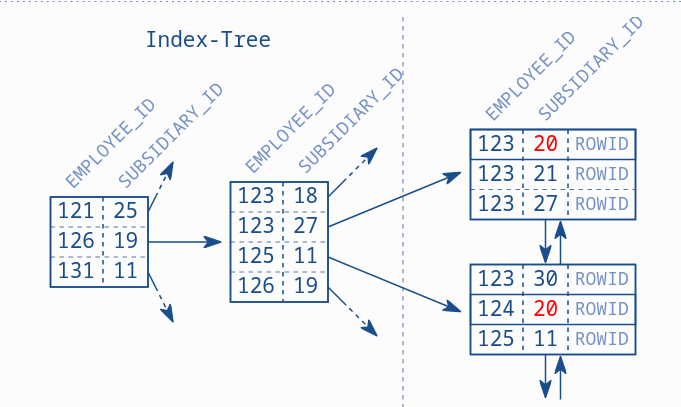
\includegraphics[width=0.7\textwidth]{btree}
    \caption{\href{https://use-the-index-luke.com/sql/where-clause/the-equals-operator/concatenated-keys}{B-Tree}}
\end{figure}
\begin{itemize}
    \item Types of indexes
    \begin{itemize}
        \item Primary index: Also known as clustered index, is a structure to store data in order usually by a primary key
        \item Secondary index: Also known as non clustered index, is an structure that provides an alternative way to access data
        \item Unique indexes
        \item Single column indexes
        \item Multi column index
        \item Bitmap index
        \item B-Tree index
        \item Function-based index
        \begin{itemize}
            \item Precomputed columns as workaround
            \item Only deterministic functions must be used
        \end{itemize}
    \end{itemize}
    \item Slow queries causes
    \begin{itemize}
        \item Not using indexes: full table scan
        \item Incorrect index design
        \begin{itemize}
            \item Long index range prefer to use full table scan
            \item Data skew: fetch many rows individually
            \item Fetch data: mainly from heap
        \end{itemize}
    \end{itemize}
    \item Tips
    \begin{itemize}
        \item Combining indexes avoid creating multiple distinct bitmap indexes
        \item Over indexing induce overhead on update/delete/insert
        \item Use non-key columns in indexes for common access patterns
        \item Index must use leftmost subset of columns
    \end{itemize}
    \item Index related operations
    \begin{itemize}
        \item Index only scan: hit index
        \item Index unique scan: retrieves single row, hit index and heap
        \item Index range scan: retrieves multiple rows, hit index and heap
        \item full table scan: hit heap
    \end{itemize}
\end{itemize}


\subsection{Reliability, Scalability and Mantainability}
\begin{definition}[Reliability]
    Keep working with hardware, software and human errors. To implement is important to decouple and isolate components, seek faults over failure, make easy to do the right thing and discourage the wrong, make fast to roll back changes.
\end{definition}
\begin{definition}[Scalability]
    Reasonable ways to deal with grows. To implement reliability is important to describe with metrics.
\end{definition}
\begin{definition}[Maintainability]
    It is divided into three parts
    \begin{itemize}
        \item Operability: Make operations easy. To implement track problem causes, automate deployment, define process.
        \item Simplicity: Easy for new engineers to understand. To implement seek abstraction over hardcode.
        \item Evolvability: Make easy for engineers to make changes.
    \end{itemize}
\end{definition}


\end{document}
